\documentclass[aspectratio=169,t,11pt]{beamer}
% \documentclass[aspectratio=43,t,11pt]{beamer}
\usepackage{slides,math}

% Define `accent`/`accent2` colors for theme customization
\definecolor{accent}{HTML}{006896}
\definecolor{accent2}{HTML}{695693}

\title{What is the Effect of X on Y?}
\date{\today}
\author{Kyle Butts}
\addbibresource{references.bib}
\begin{document}

% ------------------------------------------------------------------------------
\begin{frame}[noframenumbering,plain]
\maketitle


% \vspace{2.5mm}
% {\footnotesize $^*$ A bit of extra info here. Add an asterich to title or author}
\end{frame}
% ------------------------------------------------------------------------------

% ------------------------------------------------------------------------------
\section{Common Items}
% ------------------------------------------------------------------------------

\begin{frame}{Components}{Bullet Points \& Button}\label{main1}
  This section highlights commonly used components and their theming

  \begin{itemize}
    \item Can emphasize with \alert{the alert command}
    
    \begin{itemize}
      \item This allows you to draw attention to specific words/phrases
    \end{itemize}
    
    \item To include things in appendix, you must first label the slide and the appendix slide and then include a hyperlink. The command \texttt{\textbackslash bottomleft} will position in the bottom left corner nicely
  \end{itemize}

  \bottomleft{\hyperlink{appendix1}{\beamergotobutton{Appendix}}}
\end{frame}


\begin{frame}{Components}{Numbered Lists}
  You can also use numbered items that look a bit more professional

  \begin{enumerate}
    \item Pretty good
    
    \item To include things in appendix
  \end{enumerate}
\end{frame}

\begin{frame}{Components}{Citations}
  Topic 1: Spatial Frictions
  \citecolor{
    [\citet{Fajgelbaum_Morales_Serrato_Zidar_2018}, \citet{Hsieh_Moretti_2019}, and \citet{Moretti_2011}]
  }

  \vspace{5mm}
  Topic 2: Blah 
  \citecolor{
    [\citet{Suárez_Serrato_Zidar_2016}]
  }
\end{frame}

\begin{frame}{Components}{Blocks}
  \begin{block}{Theorem 1}
  The main specificaiton is as follows: 
  $$
    y_{it} = X_{it} \beta + \mu_i + \varepsilon_{it}
  $$
  \end{block}
\end{frame}

\begin{frame}{Components}{Blocks}
  \begin{purpleBlock}{}
    This is a purple block
  \end{purpleBlock}

  \begin{cranberryBlock}{With Title}
  This is a cranberry block
  \end{cranberryBlock}
\end{frame}

\begin{frame}{Components}{Colors}
  \navy{Test sentence with \textbackslash navy\{...\}}

  \purple{Test sentence with \textbackslash purple\{...\}}

  \orange{Test sentence with \textbackslash orange\{...\}}
  
  \teal{Test sentence with \textbackslash teal\{...\}}

  \kelly{Test sentence with \textbackslash kelly\{...\}}

  \ruby{Test sentence with \textbackslash ruby\{...\}}

  \alice{Test sentence with \textbackslash alice\{...\}}

  \daisy{Test sentence with \textbackslash daisy\{...\}}

  \coral{Test sentence with \textbackslash coral\{...\}}

  \cranberry{Test sentence with \textbackslash color\{cranbery\}}
\end{frame}

\begin{frame}{Components}{Background Colors}
  \bgNavy{Test word} with \textbackslash bgNavy\{...\}

  \bgPurple{Test word} with \textbackslash bgPurple\{...\}

  \bgOrange{Test word} with \textbackslash bgOrange\{...\}

  \bgTeal{Test word} with \textbackslash bgTeal\{...\}

  \bgKelly{Test word} with \textbackslash bgKelly\{...\}

  \bgRuby{Test word} with \textbackslash bgRuby\{...\}

  \bgAlice{Test word} with \textbackslash bgAlice\{...\}

  \bgDaisy{Test word} with \textbackslash bgDaisy\{...\}

  \bgCoral{Test word} with \textbackslash bgCoral\{...\}

  \bgCranberry{Test word} with \textbackslash bgCranberry\{...\}
\end{frame}

\begin{frame}{Components}{Two Columns}
  \begin{columns}[T]
  \begin{column}{.50\textwidth}
    \vspace{0pt}
    {\color{accent}\rule{\linewidth}{2pt}}
    Column 1

    \begin{enumerate}
      \item Bullet points for this column that can go over lines
      \item b
      \item c
    \end{enumerate}
  \end{column}
  
  \hfill
  
  \begin{column}{.50\textwidth}
    {\color{accent}\rule{\linewidth}{2pt}}
    Column 2

    \begin{itemize}
      \item a
      \item b
      \item c
    \end{itemize}
  \end{column}
  \end{columns}
\end{frame}

\begin{frame}{Components}{Two Columns with Figure}
  \begin{columns}[T]
  \vspace{0pt}
  \begin{column}{.5\textwidth}
    \includegraphics[width=\textwidth]{img/kanagawa.jpg}
  \end{column}
  \hfill
  \begin{column}{.48\textwidth}
    \begin{itemize}
    \item A point about the figure that is potentially important.
    \item Another point about the figure that is also potentially important.
    \end{itemize}
  \end{column}
  \end{columns}
\end{frame}

% ------------------------------------------------------------------------------
\section{Table}
% ------------------------------------------------------------------------------

\begin{frame}{Table}
  \begin{columns}[T]
  \begin{column}{.4\textwidth}
    \begin{adjustbox}{max width = \textwidth, center}
      \begin{tabular}{@{} l *{2}{r} @{}} 
        \toprule
        & (1) & (2)\\ 
        \midrule
        
        \only<1>{
          Handling of Complaints & 0.692$^{***}$& 0.682$^{***}$ \\ 
          &  (0.149) & (0.129) \\
        }
        \only<2>{
          \marktopleft{ex1}Handling of Complaints & 0.692$^{***}$& 0.682$^{***}$ \\ 
          &  (0.149) & (0.129) \markbottomright{ex1} \\
        }
        No Special Privileges & -0.104 & $-$0.103  \\ 
        & (0.135) & (0.129) \\
        Opportunity to Learn & 0.249 & 0.238$^{*}$ \\ 
        & (0.160) & (0.139) \\
        
        \midrule 
        Observations & 30 & 30 \\ 
        R$^{2}$ & 0.715 & 0.715 \\ 
        \bottomrule

      \end{tabular}   
    \end{adjustbox}
      
    \note{$^{*} p<0.1$; $^{**} p<0.05$; $^{***} p<0.01$.}
  \end{column}
  \hfill
  \begin{column}{.5\textwidth}
    \begin{itemize}
      \item Use \texttt{\textbackslash marktopleft\{name\}} and \texttt{\textbackslash markbottomright\{name\}} within the table to create box.
      \item Using \texttt{\textbackslash only} or \texttt{\textbackslash on} lets you conditionally display box
    \end{itemize}
  \end{column}
  \end{columns}
\end{frame}

% ------------------------------------------------------------------------------
\section{Figures}
% ------------------------------------------------------------------------------

% 4:3 ratio for figures
% or else it will have white space
\imageframe{img/kanagawa_16_9.png}

\begin{frame}{Figure}{Full-size Figures}
  You can use the command \texttt{\textbackslash imageframe\{img-path\}} and it will create a full-frame of a picture. 
  
  \begin{itemize}
  \item Ideally, your figure is the same aspect as the frame \texttt{4:3} or \texttt{16:9} or else there will be white space in one of the directions.
  \end{itemize}
\end{frame}

\begin{frame}{Figure}{}
  \begin{adjustbox}{width = 0.7\textwidth, center}
  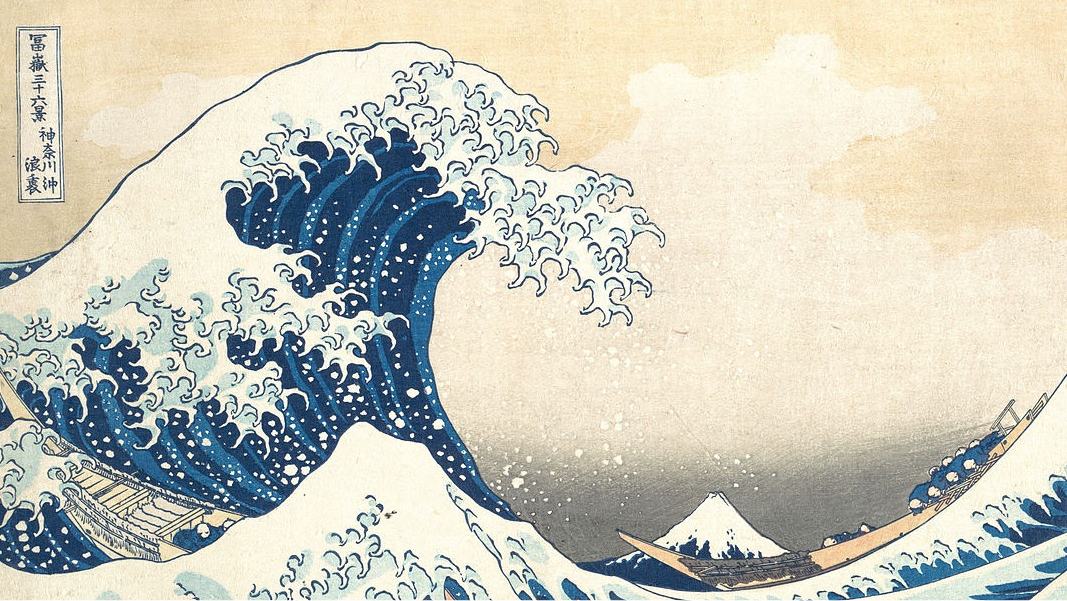
\includegraphics{img/kanagawa_16_9.png}
  \end{adjustbox}
\end{frame}

% ------------------------------------------------------------------------------
\begin{frame}[allowframebreaks,noframenumbering]{References}
  \thispagestyle{empty}
  \printbibliography
\end{frame}
\appendix
% ------------------------------------------------------------------------------

\begin{frame}{Appendix Slide}{Summary Slides}\label{appendix1}
  \begin{table}[t]
    % \caption{Summary Statistics}\label{tab:summary_stats}
    \begin{adjustbox}{width = 0.8\textwidth}
      \begin{tabular}{@{} lccccccc @{}} 
        \toprule
        Statistic & \multicolumn{1}{c}{N} & \multicolumn{1}{c}{Mean} & \multicolumn{1}{c}{St. Dev.} & \multicolumn{1}{c}{Min} & \multicolumn{1}{c}{Pctl(25)} & \multicolumn{1}{c}{Pctl(75)} & \multicolumn{1}{c}{Max} \\ 
        \hline \\[-1.8ex] 
        rating & 30 & 64.633 & 12.173 & 40 & 58.8 & 71.8 & 85 \\ 
        complaints & 30 & 66.600 & 13.315 & 37 & 58.5 & 77 & 90 \\ 
        privileges & 30 & 53.133 & 12.235 & 30 & 45 & 62.5 & 83 \\ 
        learning & 30 & 56.367 & 11.737 & 34 & 47 & 66.8 & 75 \\ 
        raises & 30 & 64.633 & 10.397 & 43 & 58.2 & 71 & 88 \\ 
        \bottomrule
      \end{tabular} 
    \end{adjustbox}
    
    \note{0.8\textwidth}{Using R base dataframe \texttt{attitude}. R base dataframe attitude. R base dataframe attitude.}
  \end{table}

  \bottomleft{\hyperlink{main1}{\beamerreturnbutton{Back}}}
  % \bottomright{\hyperlink{main1}{\beamerreturnbutton{Back}}}
\end{frame}

\end{document}
